\chapter{Grundlagen}

\section{Generalisierung}

\section{Auswahlkomponenten im Vergleich}

\begin{table}[ht!]
    \rowcolors{2}{gray!30}{gray!20}
    \caption{Vergleich der Auswahlmöglichkeiten}
    \bigskip
    \centering
    \scalebox{0.8}{
        \small
        \begin{tabular}{ p{2.5cm} || p{2.8cm} | p{3.3cm} | p{3.3cm} | p{3.3cm} }
            \TBstrut Kriterium & Buttons & Select & List & Country Input \\
            \hline % column for new goal input
            \hline
            \TBstrut Optimale Anzahl Elemente & 1 - 3 & 7 ± 2 & 70 ± 20 & ca. 250 \\
            \hline
            \TBstrut Alternativ-Name & keine & Choice Input & Combo Box & keine \\
            \hline
            \TBstrut Falsche Auswahl & \xmark & \xmark & \cmark & \xmark \\
            \hline
            \TBstrut Readonly & \cmark & \cmark & \cmark & \xmark \\
            \hline
            \TBstrut Multi-Auswahl & \cmark & \cmark & \xmark & \xmark \\
            \hline
            \TBstrut Werte-Typ & Skalar & Skalar & Skalar & Objekt \\
            \hline
            \TBstrut Aktion bei Symbol-Eingabe & keine & Sprung (Fokus) zu passendem/ nachhfolgendem Wert & Filtern der Listen-Werte & Sprung zu zuletzt passendem Wert \\
            \hline % split uo to properies
            \TBstrut Vorteile & Direkte Aktion, einfache Nutzung & Mehrfachauswahl, vordefinierte Optionen & Große Datensätze, Eingabeunterstützung, Musterprüfung & Speziell für Länderauswahl angepasst, unterstützt große Datensätze, strukturierte Objektrückgabe \\
            \hline % split uo to properies
            \TBstrut Nachteile & Begrenzte Interaktion, nicht für mehrere Auswahlmöglichkeiten geeignet & Nicht skalierbar für große Datensätze & Kann mit sehr großen Datensätzen unhandlich werden & Festgelegt auf spezifischen Anwendungsfall (Länderauswahl) \\
            \hline
            \TBstrut Anwendungen & Navigationslinks, Bestätigungsbuttons & Formularfelder mit begrenzten Auswahlmöglic & Filterbare Listen, Suchergebnis & Dropdown zur Länderauswahl in Formularen \\
            % \hline % own table for browsers
            % Bilder 
            %     & 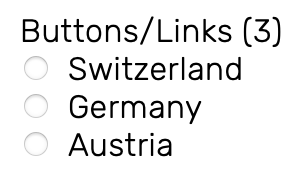
\includegraphics[width=28mm,scale=0.5]{radios-example.png} 
            %         \captionof{figure}{Radio Buttons mit 3 Werten}
            %     & 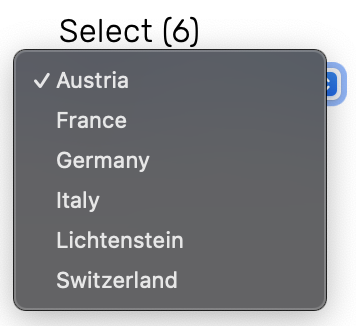
\includegraphics[width=33mm,scale=0.5]{select-open-example.png} 
            %         \captionof{figure}{Select mit 6 Werten}
            %     & 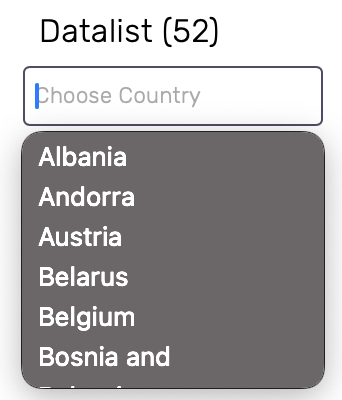
\includegraphics[width=33mm,scale=0.5]{datalist-example.png} 
            %         \captionof{figure}{Datalist mit 52 Werten}
            %     & 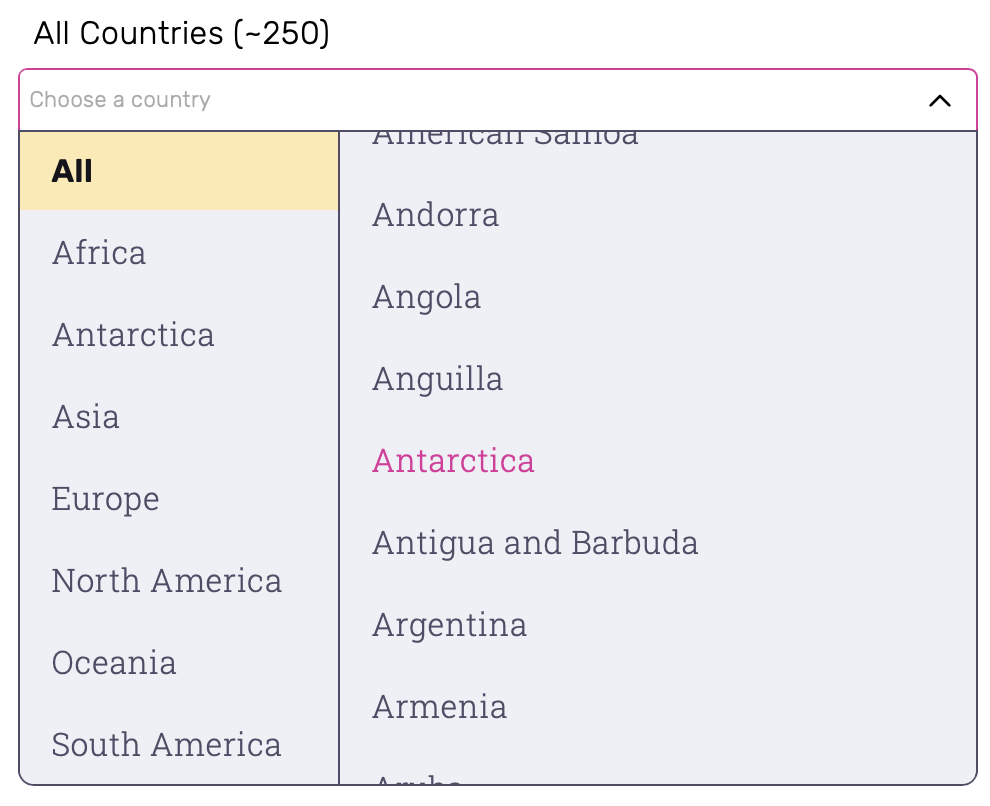
\includegraphics[width=33mm,scale=0.5]{country-list-example.png} 
            %         \captionof{figure}{Country Input}
            % \\
        \end{tabular}
    }
\end{table}

\import{../tables}{b.edge.tex}

% \import{../tables}{b.chrome.win.tex}

% \import{../tables}{b.firefox.win.tex}

% \import{../tables}{b.safari.tex}


% ----------------------------------------------------------------

% \begin{figure}[h]
%     \centering
%     
\includegraphics[width=60mm,scale=0.5]{kolibri-logo.png}
%     \caption{Kolibri Logo}
%     \label{Abbildung:Kolibri}
% \end{figure}

\cite{online}
